% !TEX encoding = UTF-8 Unicode

\documentclass{article}
\usepackage[british]{babel}
\author{Louis DESVERNOIS}
\title{%
    SAÉ3.02 \\
    \large User documentation}
% \date{9 Juin 2022}
\usepackage[left=2.5cm,right=2.5cm,top=2.5cm,bottom=2.5cm]{geometry}
\usepackage{subcaption}
\usepackage{listings}
\usepackage{minted}
\usepackage{graphicx}
\usepackage[T1]{fontenc}
\usepackage[colorlinks=true,linkcolor=black,anchorcolor=black,citecolor=black,filecolor=black,menucolor=black,runcolor=black,urlcolor=black]{hyperref}

\setcounter{tocdepth}{2} % pour la profondeur de la ToC

\usepackage{fancyhdr}
\pagestyle{fancy}
\fancyhf{}
\renewcommand{\headrulewidth}{0pt}
\rfoot{\thepage}
\lfoot{SAÉ3.02: Louis DESVERNOIS}

\setlength{\parindent}{0ex}

%\renewcommand{\listoflistingscaption}{Table des codes}
%\renewcommand{\listingscaption}{Code}

\begin{document}

\maketitle
\tableofcontents
\listoffigures
\listoflistings

\newpage
\section{Introduction}
This document is the user documentation for the remote control program made for
the SAÉ3.04. It dwells upon the server deployment and the user frontend.

\section{Server}
\subsection{Prerequisites}
The server uses the \verb|psutil| package from PyPI, either install it
system-wide using \verb|pip install psutil| or in a virtual environment with the
following commands. This package provides easy access to information such as the
CPU and RAM utilisation or IP addresses.

\begin{listing}[H]
    \begin{minted}[breaklines]{bash}
python3 -m venv .venv
source .venv/bin/activate
pip install psutil
    \end{minted}
    \caption{Creation of the virtual environment}
    \label{venv:creation}
\end{listing}

\subsection{Starting the server}
Once \verb|psutil| is installed, simply execute \verb|main.py|, the server will
by default listen on TCP port 10000, it is however possible to start the server
on another port by adding it as an attribute.

\begin{listing}[H]
    \begin{minted}[breaklines]{bash}
python3 main.py <PORT>
    \end{minted}
    \caption{Starting the server}
    \label{venv:startingserver}
\end{listing}

To ensure that the server is able to restart properly, it will try to bind to
the specified port indefinitely every ten seconds, \emph{even if the port is not
available to the user}.

\newpage
\section{Client}
\subsection{Prerequisites}
The client uses \verb|PyQT5| for its Graphical User Interface.

\subsection{Usage}
The client uses tabs to organize the multiple connection it is able to make.

\begin{figure}[H]
    \begin{center}
        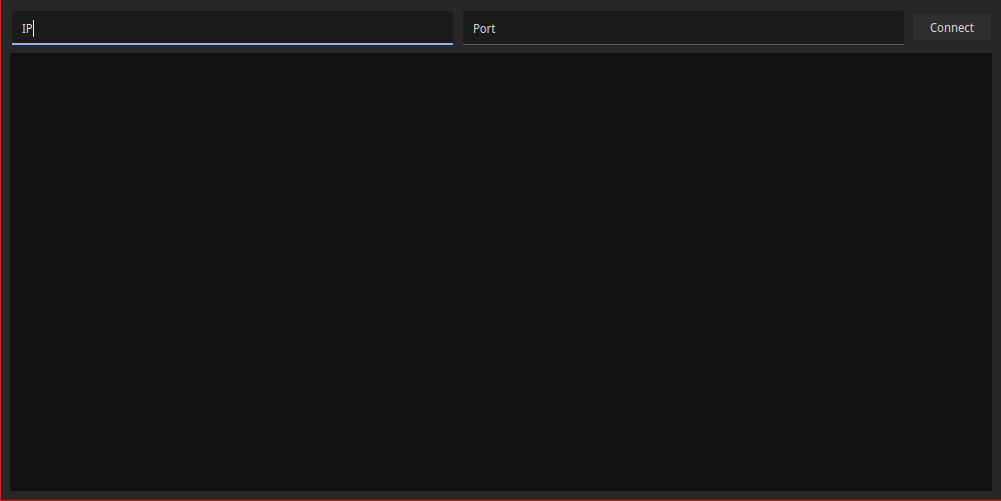
\includegraphics[width=0.8\linewidth]{fig/first.png}
    \end{center}
    \caption{Client first time launch}
    \label{client:default}
\end{figure}

To open a new connection, enter the server's IP address and port in the two
fields on top and click the "Connect" button. If the connection is successful,
this will open a new tab.

\begin{figure}[H]
    \begin{center}
        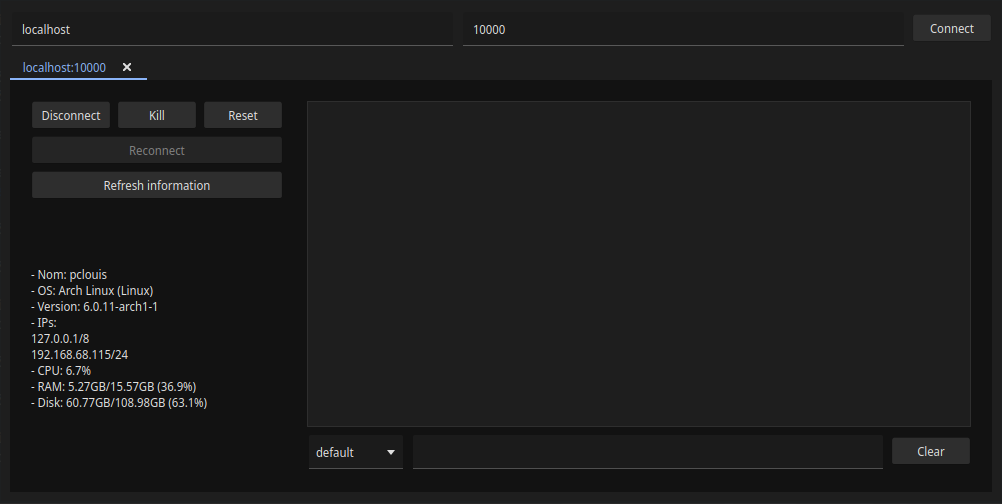
\includegraphics[width=0.8\linewidth]{fig/connected.png}
    \end{center}
    \caption{First connection}
    \label{client:connected}
\end{figure}

The interface consists of two panes, the left is the server control and the
information about the machine it is running on, the right is the "shell" to send
commands to the server.

\subsubsection{Server control and information}
\begin{figure}[H]
    \begin{center}
        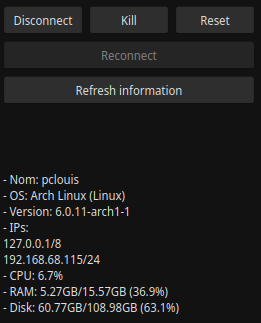
\includegraphics[width=0.25\linewidth]{fig/left.png}
    \end{center}
    \caption{Left pane}
    \label{client:left}
\end{figure}
This section is used to control the server state, the buttons allows to either
disconnect from the server\footnote{Closing the tab automatically disconnects
the client from the server}, kill the server and reset the server\footnote{This
recreates the socket on the server side, it can take up to a minute}. Once one
of these buttons are pressed, the "Reconnect" is enabled. The information about
the machine is automatically requested when the connection is created, however,
the "Refresh information" button is available as long as the client is still
connected.

\subsubsection{Server shell}
\begin{figure}[H]
    \begin{center}
        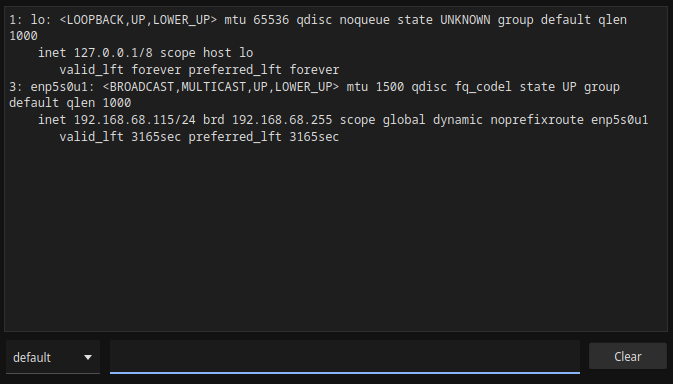
\includegraphics[width=0.7\linewidth]{fig/command.png}
    \end{center}
    \caption{Right pane}
    \label{client:right}
\end{figure}
To send a command to the server, enter the command in the field and press the
enter key. The ComboBox offers a choice of different shells, such as DOS or
PowerShell for Windows. To clear the screen, use the button next to the command
field.

\newpage
\subsection{Save servers in a CSV file}
The application is able to connect automatically on servers at startup, this is
done using the \verb|servers.csv| file. This file must be in the same directory
as the application's \verb|main.py| file. The application excepts a comma
separated list of: the server's name, IP address and port.
\begin{listing}[H]
    \begin{minted}[breaklines]{text}
dev serv,localhost,10000
test serv,localhost,10001
    \end{minted}
    \caption{Example of a CSV file expected by the client}
    \label{venv:csv}
\end{listing}
\end{document}